\documentclass[sigconf, balance, nonacm]{acmart}


\usepackage[english]{babel}
\usepackage{tikz}
\usepackage{graphviz}

%% get subsubsections in TOC
\setcounter{tocdepth}{4}


%% These commands are for a PROCEEDINGS abstract or paper.
\acmConference[WLSD 2025]{Workshop on Low-level Software Development}{June 13, 2025}{Evanston, IL}

%%
%% For managing citations, it is recommended to use bibliography
%% files in BibTeX format.
%%
%% You can then either use BibTeX with the ACM-Reference-Format style,
%% or BibLaTeX with the acmnumeric or acmauthoryear sytles, that include
%% support for advanced citation of software artefact from the
%% biblatex-software package, also separately available on CTAN.
%%
%% Look at the sample-*-biblatex.tex files for templates showcasing
%% the biblatex styles.
\bibliography{bibs/pdinda,bibs/pdinda2,bibs/fpspy,bibs/riscv,bibs/village,bibs/mw,bibs/sam-umut}

\begin{document}

%% The "title" command has an optional parameter,
%% allowing the author to define a "short title" to be used in page headers.
\title{Village Synthesis}

%% The "author" command and its associated commands are used to define
%% the authors and their affiliations.
%% Of note is the shared affiliation of the first two authors, and the
%% "authornote" and "authornotemark" commands
%% used to denote shared contribution to the research.
\author{Liam Strand}
\affiliation{%
	\institution{Northwestern University}
	\city{Evanston}
	\state{IL}
	\country{USA}
}
\email{ltrs@u.northwestern.edu}
\orcid{0009-0005-9712-1689}

\begin{abstract}
	The cell divides and a hundred million years later, it’s
	a bull shark or Sophocles. Not sure which; not sure
	how these things work. Point is:
	things change, evolve, move forward.

	You get the job, get promoted, get fired. Lead
	becomes gold, then one day it doesn’t.
	The sun orbits the earth, then one day it doesn’t.
	The whale gets legs, gets bored with land, goes back

	to the ocean, the legs are now a metaphor. Nothing certain,
	nothing written in stone that can’t be unwritten by the
	hammer. The world keeps trying to end itself because it
	wants to end, then one day it doesn’t.

	You get homesick. Get heartburn. Get a strange yearning to
	pray when looking at photographs or cellphone towers. You
	have a hard time adjusting to your new status, station, or
	impending fate. You believed one thing,

	now you believe something else. The earth has ice caps, then
	one day it doesn’t. Everything: converted
	to a newer thing. Meanwhile: old gods become lesser gods,
	become priests leaving offerings at someone else’s altar.

	The god of war grows up to sell pocketknives at a pawn shop. The
	goddess of carrots peddles sinus medications.
	The messenger god now brings your mail—
	and there he is, right on schedule, one house to the next.

	This always stuns me: the way an envelope arrives; how we still
	reach toward one another, how this correspondence endures:
	one figure approaches your door with a satchel full of sand,
	pigeon feathers, sorrows, and names.
\end{abstract}

%% Keywords. The author(s) should pick words that accurately describe
%% the work being presented. Separate the keywords with commas.
\keywords{Nested-Data Parallelism, Heterogeneity, FPGA, HDL Synthesis}

%% A "teaser" image appears between the author and affiliation
%% information and the body of the document, and typically spans the
%% page.
\begin{teaserfigure}
	\begin{center}
		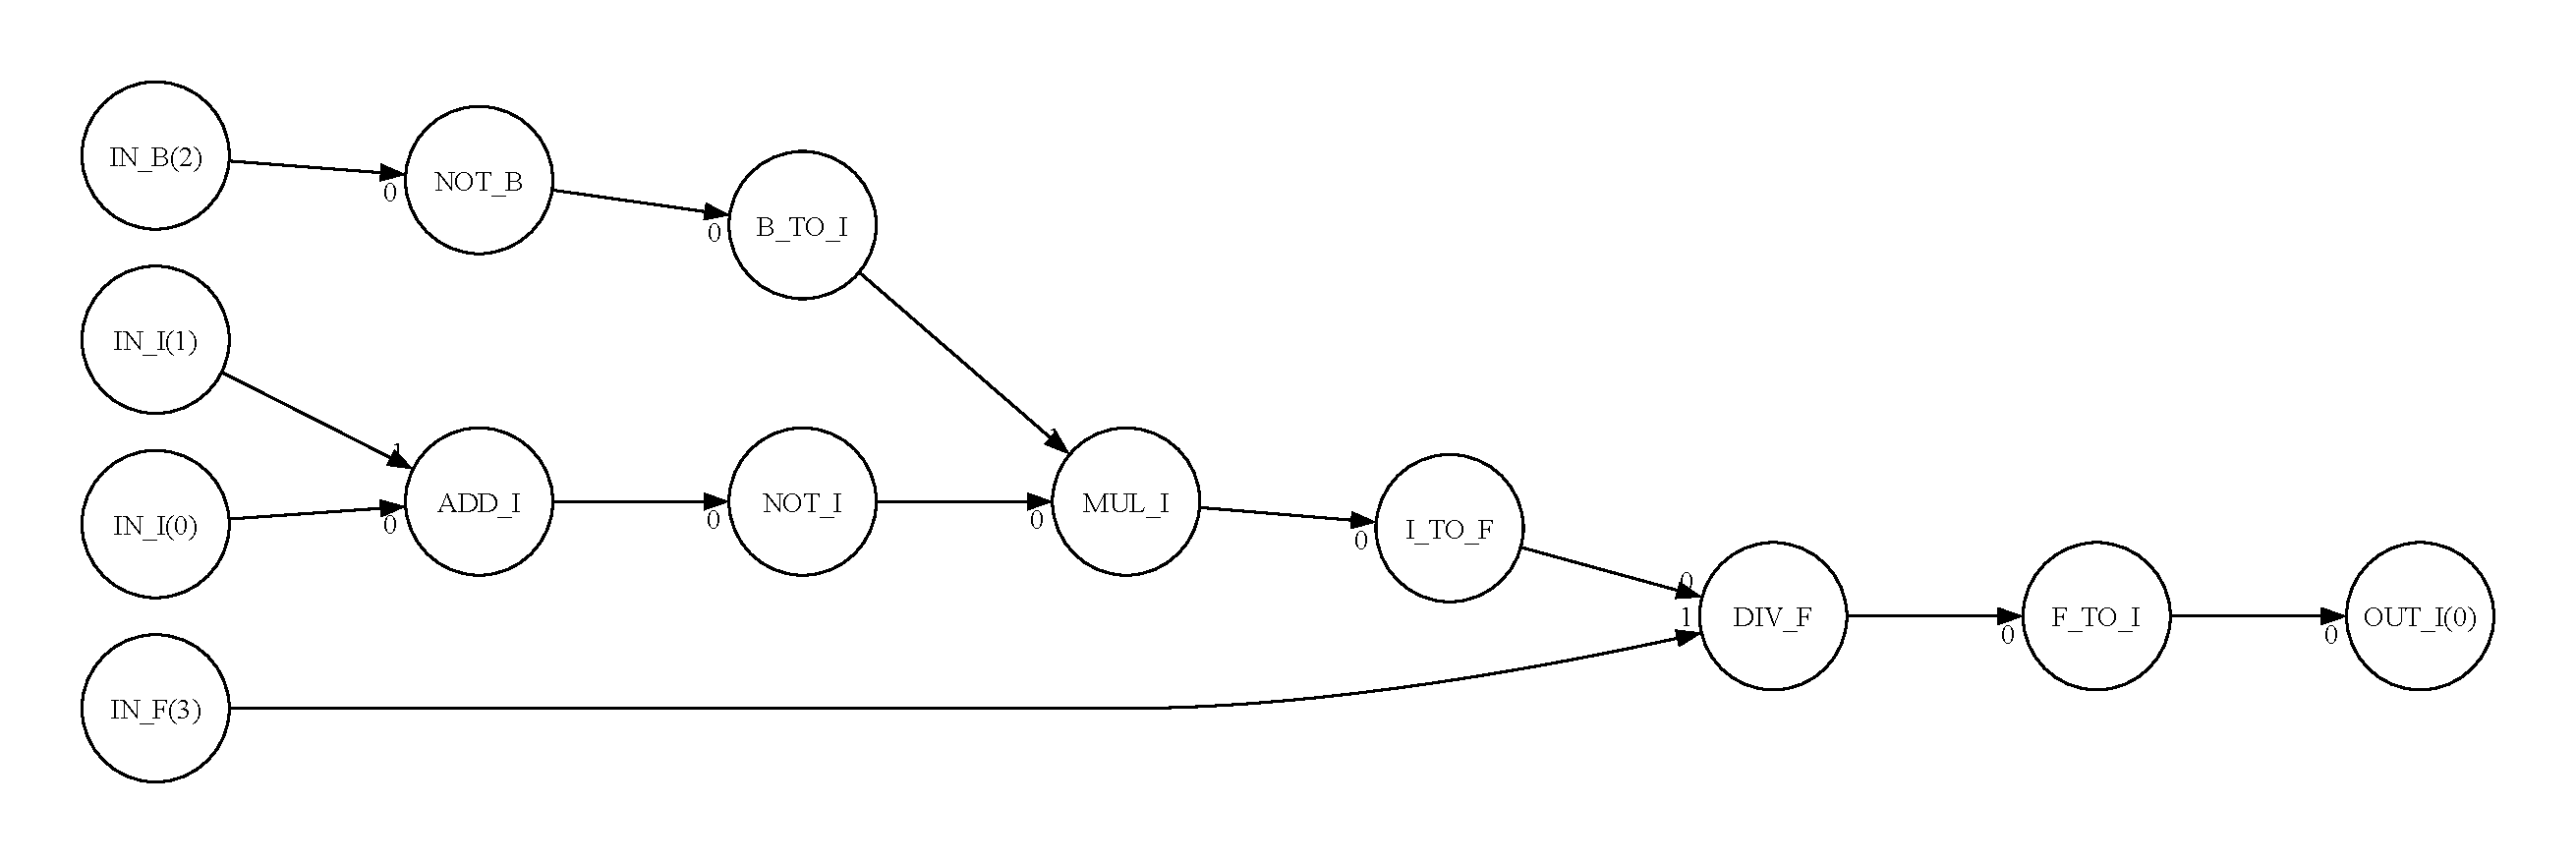
\includegraphics[width=0.95\textwidth]{figures/teaser.pdf}
		\label{fig:teaser}
		\caption{TODO}
	\end{center}
\end{teaserfigure}

% \received{13 June 2025}
% \received[Accepted]{13 June 2025}

%%
%% This command processes the author and affiliation and title
%% information and builds the first part of the formatted document.
\maketitle

\tableofcontents

\section{Introduction}

%%%%%%%%%%%%%%%%%%%%%%%%%%%%%%%%%%%%%%%%%%%%%%%%%%%%%%%%%%%%%%%%%%%%%%%%%%%%%%%%

\section{Background}

\subsection{Village}

\subsubsection{NESL}

\subsubsection{VCODE}

\subsubsection{VIR}

\subsection{Chisel}

%%%%%%%%%%%%%%%%%%%%%%%%%%%%%%%%%%%%%%%%%%%%%%%%%%%%%%%%%%%%%%%%%%%%%%%%%%%%%%%%

\section{Operator Graphs in Scala}

\subsection{Node Contents}

\subsection{\texttt{scala-graph} DSL}

\subsection{Graph Validation}

%%%%%%%%%%%%%%%%%%%%%%%%%%%%%%%%%%%%%%%%%%%%%%%%%%%%%%%%%%%%%%%%%%%%%%%%%%%%%%%%

\section{Hardware Functional Unit Library}

\subsection{Simple Unary and Binary Units}

\subsection{Input and Output}

\subsection{Floating Point with \texttt{hardfloat}}

\subsection{Conversions}

%%%%%%%%%%%%%%%%%%%%%%%%%%%%%%%%%%%%%%%%%%%%%%%%%%%%%%%%%%%%%%%%%%%%%%%%%%%%%%%%

\section{Connecting Functional Units}

\subsection{\texttt{VillageFunctionalUnit} Interface}

\subsection{Operand Buffering}

\subsection{Wiring It All Up}

\subsection{Accelerator I/O}

%%%%%%%%%%%%%%%%%%%%%%%%%%%%%%%%%%%%%%%%%%%%%%%%%%%%%%%%%%%%%%%%%%%%%%%%%%%%%%%%

\section{Results}

\subsection{Testing Approach}

\subsection{Testing Results}

%%%%%%%%%%%%%%%%%%%%%%%%%%%%%%%%%%%%%%%%%%%%%%%%%%%%%%%%%%%%%%%%%%%%%%%%%%%%%%%%

\section{Conclusion}

%%%%%%%%%%%%%%%%%%%%%%%%%%%%%%%%%%%%%%%%%%%%%%%%%%%%%%%%%%%%%%%%%%%%%%%%%%%%%%%%

\section{Future Work}

\subsection{Superscalar}

\subsection{Simulated Integration}

\subsection{Hardware Integration}

\subsection{Dynamics}


%%%%%%%%%%%%%%%%%%%%%%%%%%%%%%%%%%%%%%%%%%%%%%%%%%%%%%%%%%%%%%%%%%%%%%%%%%%%%%%%

\begin{acks}
\end{acks}

\end{document}
\endinput
